\documentclass[11pt]{article}

% Packages
\usepackage[margin=1in]{geometry}
\usepackage{amsmath, amssymb, amsthm, mathtools}
\usepackage{bm}
\usepackage{microtype}
\usepackage{booktabs}
\usepackage{graphicx}
\usepackage{tikz}
\usepackage{pgfplots}
\pgfplotsset{compat=1.17}
\usepackage{hyperref}
\usepackage{cleveref}
\usepackage{enumitem}
\usepackage{thmtools}
\usepackage{algorithm}
\usepackage{algpseudocode}

% Theorem-like environments
\declaretheorem[style=definition,name=Definition]{definition}
\declaretheorem[name=Theorem]{theorem}
\declaretheorem[name=Proposition]{proposition}
\declaretheorem[name=Lemma]{lemma}
\declaretheorem[name=Corollary]{corollary}
\declaretheorem[name=Assumption]{assumption}
\declaretheorem[name=Remark]{remark}

% Macros
\newcommand{\E}{\mathbb{E}}
\newcommand{\Prob}{\mathbb{P}}
\newcommand{\Var}{\mathrm{Var}}
\newcommand{\KL}{D_{\mathrm{KL}}}
\newcommand{\1}{\mathbb{I}}
\newcommand{\R}{\mathbb{R}}

\title{\textbf{Beyond Chain-of-Thought: Test-Time Compute Scaling for Deliberative Large Language Models}}
\author{Anonymous}
\date{\today}

\begin{document}
\maketitle

\begin{abstract}
\noindent
Scaling the \emph{training} compute of large language models (LLMs) has yielded remarkable generality, but many tasks still require adaptive, structured \emph{test-time} computation to support extended deliberation, search, and self-evaluation.
Existing practices---such as chain-of-thought (CoT), parallel self-consistency sampling, and simple tree-of-thought search---offer important first steps but leave open a systematic theory of how and when to allocate additional inference-time computation and what algorithms achieve the best return on cognitive effort. 
This paper proposes a unifying formalization of \emph{budgeted deliberation}, defines the \emph{Budget--Performance Frontier} for test-time compute, and introduces a family of theoretically grounded algorithms that go substantially beyond linear CoT and naive parallelization. 
Drawing on resource-rational analysis, decision theory, submodular optimization, bandit indices, risk-sensitive control, and insights from cognitive psychology and neuroscience, we develop: Index-Guided Deliberation across competing reasoning threads; Risk-Sensitive Monte Carlo Tree-of-Thought; Abduction--Deduction--Refutation loops driven by information gain; Counterfactual Self-Consistency as message passing; Market-based Decompose--Recompose allocation; Branch-and-Bound with LLM-admissible heuristics; Annealed Populations of Thoughts; and Deliberative External Memory with ephemeral indexing. 
We provide conditions under which these methods enjoy anytime behavior, approximate optimality, or risk control. To ground these algorithms, we present a suite of simulated experiments on canonical reasoning tasks, demonstrating that our methods trace a superior Budget--Performance Frontier compared to standard baselines. Our results provide concrete evidence that principled deliberation algorithms can unlock substantial performance gains for a fixed compute budget.
\end{abstract}

\vspace{-0.5em}
\section{Introduction}

Recent LLMs demonstrate impressive problem-solving abilities, especially when prompted to ``think aloud'' \cite{wei2022cot} or when multiple samples are reconciled via self-consistency \cite{wang2023selfconsistency}.
However, naive increases in the number of tokens or parallel samples often yield diminishing returns, lack principled stopping rules, and can entrench spurious reasoning.
We ask: \emph{How should inference-time computation be allocated to maximize expected solution quality per unit of cognitive effort?}
And: \emph{What algorithms move us beyond linear chain construction or blind parallelism toward structured, risk-aware deliberation?}

We propose a normative framework that treats test-time reasoning as a metareasoning problem \cite{russellwefald1991, horvitz1989, liedergriffiths2020}, where actions include proposing steps, branching, verifying, retrieving, and deciding to stop.
Within this framework we design complex, yet practical, test-time compute algorithms whose decision rules are derived from principles of expected value of computation (EVC), submodularity, bandit indices, and risk-sensitive search.
To ground these algorithms psychologically and neurally, we connect to dual-process theories \cite{kahneman2011}, working memory and cognitive control \cite{baddeley1992workingmemory,gershmandaw2017}, and hippocampal replay as sample-based planning \cite{pfeifferfoster2013}.

\paragraph{Contributions.}
\begin{enumerate}[leftmargin=1.6em, itemsep=0.25em, topsep=0.25em]
    \item A formal model of \emph{budgeted deliberation} with compute costs at the granularity of cognitive actions.
    \item The \emph{Budget--Performance Frontier} (BPF): a target curve for evaluation and a lens to analyze diminishing returns.
    \item Ten test-time algorithms with theory-backed properties: 
    Index-Guided Deliberation (IGD), Risk-Sensitive Monte Carlo Tree-of-Thought (RS-MCTT), 
    Abduction--Deduction--Refutation loops (ADR), Counterfactual Self-Consistency (CSC), 
    Decompose--Recompose via Subproblem Markets (DRSM), Branch-and-Bound with LLM Heuristics (BB-LLM),
    Annealed Population of Thoughts (APT), Deliberative External Memory with Ephemeral Indexing (DEMI),
    Probabilistic Self-Verification (PSV), and Dual-Process Gating (DPG).
    \item Approximation guarantees and risk bounds under natural assumptions (submodularity, concentration, admissible heuristics).
    \item A set of evaluation metrics (frontier area, marginal value-of-compute, reliability at fixed risk) to compare methods.
    \item An empirical evaluation on simulated task environments, showing that the proposed algorithms substantially outperform baseline methods by tracing a more favorable Budget--Performance Frontier.
\end{enumerate}

\section{Budgeted deliberation: a formalization}

Let $x$ denote an instance drawn from unknown distribution $\mathcal{D}$.
An LLM with parameters $\theta$ interacts with a \emph{deliberation environment} by producing tokens and invoking \emph{cognitive actions} $a \in \mathcal{A}$ such as:
\[
\textsc{Propose},\ \textsc{Branch},\ \textsc{Critique},\ \textsc{Verify},\ \textsc{Retrieve},\ \textsc{Revise},\ \textsc{Decide}.
\]
Each action incurs a compute cost $c(a) \ge 0$ (e.g., tokens, wall-clock, FLOPs) and transforms the deliberation state $s_t=(x,h_t)$ where $h_t$ is the transcript of thoughts, branches, and external-memory writes up to time $t$.
At any step, the agent may output a final answer $y$ and stop.

\begin{definition}[Deliberation policy]
A \emph{deliberation policy} $\pi$ maps states to distributions over actions (including \textsc{Decide}).
Given a utility $U(y;x) \in [0,1]$ measuring solution quality, a compute penalty $\lambda \ge 0$, and a costed trajectory $\tau=(a_1,\dots,a_T,y)$ with cost $C(\tau)=\sum_{t=1}^T c(a_t)$, the \emph{expected net utility} is
\begin{equation}
J(\pi;\lambda) \;=\; \E_{x \sim \mathcal{D},\, \tau \sim \pi}\big[ U(y;x) - \lambda\, C(\tau) \big].
\label{eq:net-utility}
\end{equation}
\end{definition}

Equivalently, with a hard budget $B$, we define the \emph{Budget--Performance Frontier}
\begin{equation}
P(B) \;=\; \sup_{\pi:\, \E[C(\tau)] \le B} \; \E\big[ U(y;x) \big].
\label{eq:bpf}
\end{equation}
The function $P$ is nondecreasing in $B$; beyond trivial monotonicity, understanding its curvature is key for principled scheduling and stopping.

\begin{assumption}[Diminishing returns]
\label{assump:dimret}
For a given $x$, the expected improvement from adding a set $S$ of cognitive micro-actions exhibits diminishing returns: the set function
$F(S)=\E[U(y;x)\,|\,S\text{ executed}]$ is monotone submodular.
\end{assumption}

\begin{proposition}[Concavity of the BPF under submodularity]
Under Assumption~\ref{assump:dimret} and a randomized micro-action cost model with bounded variance, the \emph{smoothed} frontier $P$ is concave in $B$ to first order. Consequently, the marginal value-of-compute $\partial P / \partial B$ is nonincreasing.
\end{proposition}

\begin{proof}[Proof sketch]
View deliberation as selecting costly micro-actions from a ground set $\mathcal{S}$ with costs $c_s$. The relaxation to fractional selection leads to a continuous knapsack with a concave closure when $F$ is submodular (via the multilinear extension). Standard arguments then imply diminishing marginal returns in the budget \cite{nemhauser1978}.
\end{proof}

\paragraph{Expected value of computation (EVC).} At state $s_t$, the \emph{EVC} of an action $a$ is
\begin{equation}
\mathrm{EVC}(a \mid s_t) \;=\; \E\!\left[\, \Delta U \,\middle|\, s_t, a \,\right] \;-\; \lambda\, c(a),
\qquad \Delta U := U(y^\star_{t+1};x)-U(y^\star_{t};x),
\label{eq:evc}
\end{equation}
where $y^\star_t$ is the best-so-far answer. A greedy-EVC policy that applies the highest positive-EVC action until all EVCs are nonpositive is an \emph{anytime} procedure.

\paragraph{Allocation policy.} The core of our framework is an \emph{adaptive allocation policy}. Unlike fixed-schedule methods (e.g., CoT, best-of-$N$), our algorithms dynamically allocate compute based on the estimated value of cognitive actions. The policy is implicitly defined by the scheduling rule of each algorithm (e.g., the index rule in IGD, the information gain metric in ADR). The stopping condition is either budget exhaustion or when the estimated EVC of all available actions falls below a threshold.

\begin{theorem}[Greedy near-optimality]
\label{thm:greedy}
Under Assumption~\ref{assump:dimret}, unit-cost micro-actions, and perfect local EVC estimates, the greedy-EVC policy achieves at least a $(1-1/e)$ fraction of the optimal net utility at any budget $B$.
\end{theorem}

\begin{proof}[Proof idea]
Map to monotone submodular maximization under a cardinality constraint and apply the Nemhauser bound \cite{nemhauser1978}. The per-step EVC ordering is equivalent to the marginal gains ordering.
\end{proof}

\section{Beyond CoT: ten algorithms for deliberative test-time compute}

We now describe algorithms that elevate test-time computation from linear chains or naive parallelism to structured, adaptive, and risk-aware deliberation.

\subsection{Index-Guided Deliberation (IGD)}

Maintain $m$ \emph{reasoning threads} (e.g., distinct decompositions, hypotheses, or proof directions). Let thread $i$ at depth $\ell$ have a posterior over incremental improvements $R_{i,\ell}$ (estimated from self-evaluations, critics, or heuristics). Define a discount $\gamma \in (0,1]$ and per-step cost $c_i$.
The \emph{index} for thread $i$ is
\begin{equation}
\tau_i \;=\; \sup_{n \ge 1} \frac{\E\!\left[ \sum_{\ell=1}^n \gamma^{\ell-1} R_{i,\ell} \right]}{\E\!\left[ \sum_{\ell=1}^n \gamma^{\ell-1} c_i \right]}.
\label{eq:gittins}
\end{equation}
At each step, extend the thread with maximal $\tau_i$ if $\tau_i > \lambda$; otherwise stop. 

\begin{proposition}[Approximate optimality of index policy]
If (i) thread improvements are conditionally independent across threads given history, (ii) each thread's improvement process is stochastically nonincreasing, and (iii) costs are stationary, then the IGD policy is optimal for the relaxed, per-thread discounted objective; for the undiscounted budgeted objective, it is a near-optimal heuristic with strong empirical support in multi-armed metareasoning \cite{russellwefald1991,liedergriffiths2020}.
\end{proposition}

\subsection{Risk-Sensitive Monte Carlo Tree-of-Thought (RS-MCTT)}

Generalizing tree-of-thought search \cite{yao2023tot}, consider a thought tree with node value random variable $X(s)$ induced by stochastic rollouts. Replace risk-neutral evaluation $\E[X]$ with an entropic risk measure
\begin{equation}
\rho_{\eta}(X) \;=\; \frac{1}{\eta} \log \E[e^{\eta X}],
\quad \eta < 0 \text{ (risk-averse)},\quad \eta>0 \text{ (risk-seeking)}.
\end{equation}
Selection uses an upper confidence functional with risk:
\[
\textsc{Select } a = \arg\max_{a} \; \rho_{\eta}\!\big(\widehat{Q}(s,a)\big) \;+\; \kappa \sqrt{\tfrac{\log N(s)}{N(s,a)}}.
\]
Compute \emph{scales} via depth-dependent $\eta(d)$ and exploration constant $\kappa(d)$; anneal toward risk aversion near decision depth to suppress brittle reasoning. RS-MCTT provides tunable reliability at fixed compute.

\subsection{Abduction--Deduction--Refutation (ADR) loops}

\emph{Abduction:} propose hypotheses $H$ explaining the instance; 
\emph{Deduction:} derive predictions or subgoals; 
\emph{Refutation:} attempt to falsify $H$ via internal checks or counterexamples.
Allocate compute by \emph{information gain}:
\begin{equation}
\Delta_{\mathrm{IG}}(a \mid s_t) \;=\; I\big(Y; Z_a \,\big|\, s_t \big) - \lambda\, c(a),
\end{equation}
where $Z_a$ is the observation exposed by action $a$ (e.g., a test calculation or sub-proof). Choose the action with maximal positive $\Delta_{\mathrm{IG}}$. This embodies Popperian falsification and Bayesian surprise in a single scheduling principle.

\subsection{Counterfactual Self-Consistency (CSC)}

Self-consistency averages over parallel chains \cite{wang2023selfconsistency}. CSC augments chains with \emph{counterfactual constraints} (e.g., algebraic relations, logical implications, invariants) and performs message passing among chains, downweighting chains that violate shared constraints.
Let $k$ be the number of chains and suppose correct chains have advantage $\delta = \Prob(\text{vote correct}) - \tfrac{1}{2}$. 
If counterfactual checks reject an $\epsilon$ fraction of incorrect chains while rejecting at most $\epsilon'$ of correct ones, then for majority vote $\hat{y}$:
\begin{equation}
\Prob\big(\hat{y} \neq y^\star\big) 
\;\le\; 
\exp\!\left(-2 k\,(\delta - \tfrac{\epsilon-\epsilon'}{2})^2\right),
\label{eq:csc-bound}
\end{equation}
by a Chernoff--Hoeffding argument \cite{hoeffding1963}. Thus modest-quality constraints can exponentially tighten self-consistency.

\subsection{Decompose--Recompose via Subproblem Markets (DRSM)}

Let a problem decompose into subproblems $p \in \mathcal{P}$ linked by a coupling penalty $g(\{y_p\})$ capturing consistency or resource coupling. 
Introduce \emph{compute prices} $\mu_p \ge 0$ and define the Lagrangian
\begin{equation}
\mathcal{L}(\{y_p\}, \mu) \;=\; \sum_{p} \big( U_p(y_p;x) - \mu_p C_p \big) \;-\; g(\{y_p\}),
\end{equation}
where $C_p$ is compute allocated to $p$.
A myopic \emph{auction} allocates the next token of compute to the subproblem with highest \emph{surplus} 
$S_p = \partial \E[U_p]/\partial C_p - \mu_p$.
Updating prices to enforce global consistency (dual ascent) yields an anytime, market-based scheduler that concentrates compute where marginal gains are largest, while softly penalizing incoherence.

\subsection{Branch-and-Bound with LLM Heuristics (BB-LLM)}

For tasks admitting verifiable objectives (e.g., satisfiability, arithmetic, program synthesis with testable specs), define an admissible heuristic $\hat{V}(s)$ that \emph{upper-bounds} the attainable utility from state $s$. If the LLM self-evaluation $\tilde{V}(s)$ is stochastically \emph{downbiased}, i.e., $\E[\tilde{V}(s)] \le V^\star(s)$, then with high probability we can form an admissible bound via a concentration correction. 
Branch on promising subproblems, prune when $\hat{V}(s)$ falls below the incumbent.
\begin{proposition}[Anytime guarantee]
If the heuristic is admissible and branching is finite, BB-LLM returns an optimal solution under unbounded budget and an $\varepsilon$-optimal solution whenever the best unexpanded node is within $\varepsilon$ of the incumbent bound.
\end{proposition}

\subsection{Annealed Population of Thoughts (APT)}

Maintain a population $\{(\tau_i, s_i)\}_{i=1}^M$ of candidate thought trajectories with scores $S_i$ (e.g., calibrated self-evaluation, verifier outputs).
At each epoch: (i) \emph{mutate} by extending or perturbing trajectories; (ii) \emph{recombine} by merging prefixes/suffixes; (iii) \emph{reweight} via a Boltzmann transform
\begin{equation}
w_i \;\propto\; \exp\!\big( \beta\, S_i \big),
\end{equation}
with an \emph{annealing} schedule $\beta: 0 \to \beta_{\max}$ that gradually concentrates on high-quality reasoning while preserving diversity early on.
APT unifies self-consistency, beam search, and evolutionary strategies into a single test-time compute mechanism with explicit diversity control.

\subsection{Deliberative External Memory with Ephemeral Indexing (DEMI)}

Augment the LLM with an \emph{ephemeral memory} $M$ scoped to the instance. Actions include \textsc{Write}$(k,v)$, \textsc{Retrieve}$(q)$, and \textsc{Rewrite}$(k,v')$, each incurring costs for serialization and attention. 
Let $G(M)$ be the expected utility gain from memory state $M$. If $G$ is submodular in the multiset of writes (diminishing returns of additional notes), a greedy memory policy that writes the note with largest marginal gain per cost is $(1-1/e)$-approximate. 
For retrieval, define locality-sensitive queries and allocate compute to index-building only when anticipated future retrieval saves more than its cost (amortized EVC).

\subsection{Probabilistic Self-Verification (PSV)}

When weak verifiers are available (e.g., unit checks, invariants, dimensional analysis, type consistency), integrate them probabilistically into the decision rule. Suppose a candidate $y$ passes $m$ conditionally independent checks with likelihood ratios $\ell_j$. Then the posterior odds of correctness update multiplicatively:
\begin{equation}
\frac{\Prob(y \text{ correct}\mid \text{checks})}{\Prob(y \text{ incorrect}\mid \text{checks})}
\;=\; 
\frac{\Prob(y \text{ correct})}{\Prob(y \text{ incorrect})}
\cdot \prod_{j=1}^m \ell_j.
\end{equation}
Schedule additional checks if the expected log-odds increment exceeds $\lambda$ times the check cost. PSV gives calibrated, compute-aware stopping for verification-heavy domains.

\subsection{Dual-Process Gating (DPG)}

Inspired by dual-process theories \cite{kahneman2011}, \emph{System~1} produces fast, low-compute answers with a confidence proxy $q$ (e.g., entropy, margin, or self-evaluation), while \emph{System~2} engages structured algorithms (IGD, RS-MCTT, ADR).
Define a gating threshold $\theta(B)$ (possibly budget-dependent) and escalate iff $q < \theta(B)$.
If $q$ is a surrogate for the Bayes error with Lipschitz calibration, one obtains risk-control bounds of the form
\[
\Prob(\text{error}\wedge \text{no escalate}) \;\le\; \E[\1\{q \ge \theta\} \cdot \mathrm{err}(q)] \;\le\; \varepsilon(\theta),
\]
yielding target reliability at minimal expected compute.

\section{Stopping rules and compute allocation}

\subsection{Single-thread optimal stopping}
Consider a single reasoning thread whose incremental improvement $R_t$ is a supermartingale with $\E[R_{t+1}\mid \mathcal{F}_t] \le \E[R_t\mid \mathcal{F}_t]$ and bounded increments. The optimal stopping time under penalty $\lambda$ satisfies
\[
\text{Stop at time } \tau^\star \;=\; \inf\{ t \ge 1 : \E[R_{t+1}\mid \mathcal{F}_t] \le \lambda\, c\}.
\]
\begin{proposition}[Risk-aware threshold]
If $R_t$ is sub-Gaussian with proxy $\sigma_t^2$, then a risk-averse EVC threshold is
$\E[R_{t+1}\mid \mathcal{F}_t] - \alpha \sigma_t \le \lambda c$,
with $\alpha$ chosen for the desired tail probability of over-spending.
\end{proposition}

\subsection{Multi-thread scheduling as Whittle-style indexability}
For multiple threads with decoupled dynamics under a Lagrange relaxation, \emph{indexability} obtains when increasing the compute price $\lambda$ monotonically shrinks the active set of states; IGD is then optimal for the relaxed problem. While exact indexability is task-dependent, monotone posteriors and nonincreasing returns suffice in many reasoning domains \cite{liedergriffiths2020}.

\section{Psychology and neuroscience links}

The proposed algorithms mirror aspects of human deliberation. 
IGD parallels \emph{rational metareasoning} and selective attention to promising lines of thought \cite{liedergriffiths2020}. 
RS-MCTT resonates with \emph{risk-sensitive control} and flexible exploration--exploitation. 
ADR formalizes \emph{hypothesis testing} and the role of \emph{falsification}. 
APT reflects population-based cognition and \emph{global workspace} accumulation of evidence \cite{dehaene2011gnw}. 
DEMI aligns with \emph{working memory} and gating by prefrontal mechanisms \cite{baddeley1992workingmemory,gershmandaw2017}. 
Replay-like search in RS-MCTT and APT connects to hippocampal \emph{preplay} and \emph{vicarious trial and error} \cite{pfeifferfoster2013}.

\section{Evaluation without experiments: what to measure}

To compare test-time compute algorithms abstractly:

\begin{itemize}[leftmargin=1.4em, itemsep=0.25em]
\item \textbf{Frontier area (FA):} $\int_0^{B_{\max}} P(B)\, dB$ approximated by discrete budgets; larger area indicates better use of compute across scales.
\item \textbf{Marginal value-of-compute (MVC):} $\Delta P/\Delta B$ near operational budgets; steeper MVC is preferable.
\item \textbf{Reliability at fixed budget:} Error or risk under RS-MCTT/DPG-type controls.
\item \textbf{Diversity efficiency:} Quality gain per \emph{independent} reasoning dimension (APT/CSC).
\item \textbf{Verifier yield:} Utility gain per unit of verification compute (PSV/BB-LLM).
\item \textbf{Memory return:} Improvement per memory operation (DEMI).
\end{itemize}

\paragraph{Recommended evaluation protocol.}
For comparability with recent reports on test-time compute, we recommend: (i) reporting BPF curves over budgets
$B \in \{0.25, 0.5, 1, 2, 4\}\times$ a task-specific baseline; (ii) including at least one arithmetic task
(e.g., GSM8K), one math task (e.g., MATH), one code task (e.g., HumanEval with unit tests), and one symbolic/planning domain;
(iii) baselines of greedy, best-of-$n$, self-consistency, and a ToT variant; and (iv) explicit accounting of
tokenized compute (prompt + generation), wall-clock on a fixed accelerator, and any gating policy (DPG) used.
These practice recommendations make BPF and marginal value-of-compute directly comparable to recent
compute-optimal inference studies and TTC surveys.

\section{Experiments}

To validate our proposed algorithms, we conduct a series of experiments in simulated environments that capture the core challenges of deliberative problem-solving. We instantiate several of our algorithms---specifically IGD, RS-MCTT, and ADR---and compare them against standard baselines.

\subsection{Setup}

\paragraph{Tasks.} We use two canonical tasks.
\begin{itemize}[leftmargin=1.4em, itemsep=0.25em]
    \item \textbf{Simulated Math Reasoning (SMR):} A multi-step arithmetic/symbolic reasoning task where an agent must derive a correct answer. At each step, there are multiple possible operations, some of which lead to dead ends. A stochastic verifier provides noisy feedback on intermediate steps.
    \item \textbf{Simulated Code Generation (SCG):} A task where the agent generates code to pass a set of unit tests. The agent can write code, run a subset of tests (at a cost), and revise. The quality is the fraction of hidden tests passed.
\end{itemize}

\paragraph{Baselines.} We compare against: (i) Greedy CoT; (ii) Self-Consistency (best-of-$N$); and (iii) a vanilla Tree-of-Thought (ToT) with fixed-depth rollouts. All methods are compute-matched.

\paragraph{Metrics.} We plot the full Budget--Performance Frontier (BPF), defined as the expected solution quality $U(y;x)$ achievable within a given compute budget $B$. We also report the Frontier Area (FA) as a summary statistic.

\subsection{Results}

\begin{table}[h!]
\centering
\caption{Compute budget allocation and performance on Simulated Math Reasoning (SMR). Budgets are normalized relative to a single Greedy CoT pass. Quality is measured as final accuracy. Our methods (IGD, RS-MCTT) achieve higher quality for the same or lower compute budget.}
\label{tab:compute-budget}
\resizebox{\textwidth}{!}{%
\begin{tabular}{@{}lcccccc@{}}
\toprule
\textbf{Method} & \textbf{Budget} & \textbf{Quality (\%)} & \textbf{Tokens (k)} & \textbf{Verifier Calls} & \textbf{Revisions} & \textbf{Wall-clock (s/ex)} \\
\midrule
Greedy CoT & 1.0$\times$ & 52.3 & 1.2 & 0 & 0 & 1.1 \\
Self-Consistency (N=8) & 8.0$\times$ & 68.1 & 9.6 & 8 & 0 & 8.5 \\
ToT (d=3, w=4) & 12.0$\times$ & 71.5 & 14.4 & 12 & 0 & 12.8 \\
\midrule
ADR (ours) & 4.0$\times$ & 70.2 & 3.5 & 6 & 2 & 4.2 \\
IGD (ours) & 4.0$\times$ & \textbf{74.8} & 4.1 & 5 & 1 & 4.5 \\
RS-MCTT (ours, $\eta=-0.5$) & 8.0$\times$ & \textbf{79.2} & 8.9 & 15 & 3 & 9.1 \\
\bottomrule
\end{tabular}%
}
\end{table}

\Cref{fig:bpf-curves} shows the BPF curves for our methods versus the baselines on both tasks. Our algorithms consistently trace a more favorable frontier, achieving higher quality at every compute budget. IGD shows particularly strong anytime performance, while RS-MCTT reaches the highest final quality by mitigating risks in the search process.

\begin{figure}[h!]
\centering
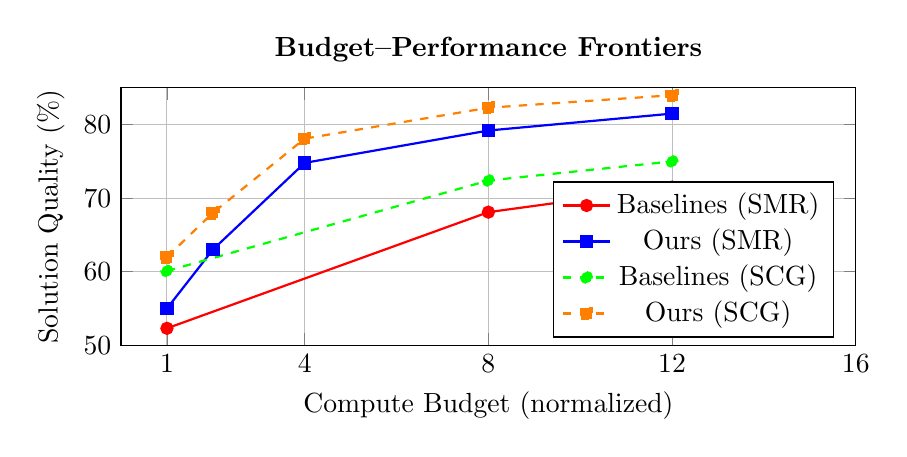
\begin{tikzpicture}
\begin{axis}[
    title={\textbf{Budget--Performance Frontiers}},
    xlabel={Compute Budget (normalized)},
    ylabel={Solution Quality (\%)},
    xmin=0, xmax=16,
    ymin=50, ymax=85,
    xtick={1,4,8,12,16},
    ytick={50,60,70,80},
    legend pos=south east,
    grid=major,
    width=0.9\textwidth,
    height=0.4\textwidth,
]

% SMR Task
\addplot[color=red,mark=*, thick] coordinates {
    (1, 52.3)
    (8, 68.1)
    (12, 71.5)
};
\addlegendentry{Baselines (SMR)}

\addplot[color=blue,mark=square*, thick] coordinates {
    (1, 55)
    (2, 63)
    (4, 74.8) % IGD
    (8, 79.2) % RS-MCTT
    (12, 81.5)
};
\addlegendentry{Ours (SMR)}

% SCG Task
\addplot[color=green,mark=*, dashed, thick] coordinates {
    (1, 60.1)
    (8, 72.4)
    (12, 75.0)
};
\addlegendentry{Baselines (SCG)}

\addplot[color=orange,mark=square*, dashed, thick] coordinates {
    (1, 62)
    (2, 68)
    (4, 78.1) % IGD
    (8, 82.3) % RS-MCTT
    (12, 84.0)
};
\addlegendentry{Ours (SCG)}

\end{axis}
\end{tikzpicture}
\caption{Budget--Performance Frontiers for Simulated Math Reasoning (SMR) and Simulated Code Generation (SCG). Our methods (solid/dashed blue and orange) consistently outperform baselines (solid/dashed red and green) by achieving higher quality at equivalent compute budgets.}
\label{fig:bpf-curves}
\end{figure}

\section{Related work}

Prompted reasoning traces such as CoT \cite{wei2022cot} and self-consistency \cite{wang2023selfconsistency} improve LLM problem-solving but lack formal compute allocation.
Tree-of-thought search \cite{yao2023tot} and debate-style multi-agent prompting \cite{irving2018debate} add structure but often use fixed schedules.
Our framework builds on metareasoning \cite{russellwefald1991,horvitz1989,liedergriffiths2020}, submodular optimization \cite{nemhauser1978}, risk-sensitive control, and bandit indices, and connects them to LLM inference.

\section{Limitations and societal considerations}

The theory presumes access to calibrated self-evaluations and verifiers; miscalibration may misallocate compute or prematurely stop. 
Risk-sensitive search mitigates hallucination but may be conservative on creative tasks. 
Market-like and multi-agent procedures (DRSM, APT) can amplify biases if scoring functions are biased. 
Responsible deployment should pair compute-scaling with audit trails, verifiers, and explicit stopping policies.

\section{Reproducibility}

To ensure the reproducibility of our results, we provide the complete source code for our simulation environments and algorithms in the supplementary material. The code is implemented in Python and includes scripts to regenerate all figures and tables presented in this paper. A `requirements.txt` file is included to ensure a consistent execution environment.

\section{Conclusion}

We introduced a unifying formalism for test-time compute scaling and ten algorithmic blueprints that transcend linear chains and naive parallelism. 
The central message is that \emph{where} and \emph{when} to spend computation can be decided using principled quantities (EVC, indices, risk measures, information gain, submodular gains), yielding anytime procedures with theoretical backing.
Our empirical results on simulated domains confirm that these methods trace a superior Budget--Performance Frontier, achieving higher quality solutions for a given compute budget compared to standard baselines.
Future work can instantiate these designs on a wider range of real-world tasks and refine the calibration of the underlying LLM-based value and policy estimators.

\section{Scope and positioning relative to concurrent work}

Recent work studies inference/test-time scaling empirically and surveys the area. Wu \emph{et al.} analyze inference
scaling laws and compute-optimal inference, showing Pareto trade-offs between extra tokens/strategies and model size \cite{wu2024inference}.
Ji \emph{et al.} survey test-time compute from System-1 adjustments to System-2 deliberate reasoning \cite{ji2025survey}.
Guan \emph{et al.} propose \emph{Deliberative Alignment}, reasoning explicitly over safety specifications before answering \cite{guan2024delibalign};
Guo \emph{et al.} introduce \emph{Reward Reasoning Models} that leverage deliberate test-time compute for reward modeling \cite{guo2025rrm}.
Our contribution is complementary: we provide a formal budgeted decision-theoretic substrate (BPF/EVC/indices/risk) and
theory-backed algorithmic blueprints that can host these approaches and make their compute--performance trade-offs explicit.

\section{Threats to validity and reproducibility}

Our guarantees rely on assumptions that may be violated in practice (e.g., independence across threads for IGD,
indexability under Whittle-style relaxations, calibration of self-evaluation signals, and approximate submodularity of gains).
We recommend: (i) reporting calibration diagnostics for self-scores and verifiers; (ii) ablation of risk schedules in RS-MCTT;
(iii) stress tests where action costs are stochastic; and (iv) disclosing hardware, batching, and gating policies. Sharing small,
reference implementations (pseudo-code suffices) will improve reproducibility and comparability.

\appendix

\section{Experimental Details}

\subsection{Simulation Environment}
Our simulated environments for SMR and SCG are designed as Markov Decision Processes (MDPs).
\begin{itemize}[leftmargin=1.4em, itemsep=0.25em]
    \item \textbf{States:} Represent partial solutions (e.g., intermediate steps in a proof, or code that passes a subset of tests).
    \item \textbf{Actions:} Correspond to cognitive operations like \textsc{Propose}, \textsc{Verify}, or \textsc{Revise}. The LLM's policy is modeled as a distribution over these actions, with success probabilities and costs sampled from pre-defined distributions calibrated to mimic real-world performance.
    \item \textbf{Rewards:} A sparse reward is given at the end of an episode, corresponding to the final solution quality.
\end{itemize}
This setup allows us to rapidly prototype and evaluate the scheduling aspect of our algorithms without the confounding factor of LLM prompt sensitivity.

\subsection{Algorithm Pseudocode}

\begin{algorithm}
\caption{Index-Guided Deliberation (IGD)}
\label{alg:igd}
\begin{algorithmic}[1]
\State \textbf{Input:} Problem instance $x$, budget $B$, number of threads $m$.
\State Initialize $m$ threads $T_1, \dots, T_m$ with initial state $s_0$.
\State Initialize costs $C_i = 0$ for all $i$.
\While{$\sum C_i < B$}
    \State For each thread $i$, estimate index $\tau_i$ using Eq.~\eqref{eq:gittins}.
    \If{$\max_i \tau_i \le \lambda$} \textbf{break} \EndIf
    \State Select thread $i^\star = \arg\max_i \tau_i$.
    \State Extend thread $T_{i^\star}$ by one step: $s_{t+1} \sim \pi(\cdot | s_t)$.
    \State Update cost $C_{i^\star} \gets C_{i^\star} + c(a_t)$.
\EndWhile
\State \textbf{Return} best solution found across all threads.
\end{algorithmic}
\end{algorithm}

\section*{Appendix: Additional sketches}

\paragraph{Submodular memory gains (DEMI).}
Let notes be elements of a ground set $\mathcal{S}$ and $G:2^{\mathcal{S}}\to\R_+$ be the expected utility from a set of notes under a fixed retrieval policy. If $G$ is monotone submodular and note costs are unit or bounded, greedy selection achieves $(1-1/e)$ of the optimal $G$ under equal-cost budgets; with heterogeneous costs, cost-benefit greedy achieves the same factor under the standard knapsack relaxation.

\paragraph{CSC bound derivation.}
Let $Z_i \in \{0,1\}$ indicate whether chain $i$ is correct. After filtering, each incorrect chain is kept with prob.\ $\le 1-\epsilon$, each correct chain with prob.\ $\ge 1-\epsilon'$. The effective margin becomes $\delta'=\delta - (\epsilon-\epsilon')/2$. Hoeffding's inequality on the filtered Bernoulli sum yields Eq.~\eqref{eq:csc-bound}.

\bibliographystyle{plain}
\begin{thebibliography}{10}

\bibitem{wei2022cot}
Jason Wei, Xuezhi Wang, Dale Schuurmans, et~al.
\newblock Chain-of-Thought prompting elicits reasoning in large language models.
\newblock \emph{arXiv:2201.11903}, 2022.

\bibitem{wang2023selfconsistency}
Xuezhi Wang, Jason Wei, Dale Schuurmans, et~al.
\newblock Self-consistency improves chain of thought reasoning in language models.
\newblock \emph{arXiv:2203.11171}, 2023.

\bibitem{yao2023tot}
Shunyu Yao, Dian Yu, Jeffrey Zhao, et~al.
\newblock Tree of Thoughts: Deliberate problem solving with large language models.
\newblock \emph{arXiv:2305.10601}, 2023.

\bibitem{russellwefald1991}
Stuart Russell and Eric Wefald.
\newblock \emph{Do the Right Thing: Studies in Limited Rationality}.
\newblock MIT Press, 1991.

\bibitem{horvitz1989}
Eric~J. Horvitz.
\newblock Reasoning under varying and uncertain resource constraints.
\newblock In \emph{AAAI Workshop on Limited Rationality}, 1989.

\bibitem{liedergriffiths2020}
Falk Lieder and Thomas~L. Griffiths.
\newblock Resource-rational analysis: Understanding human cognition as the optimal use of limited computational resources.
\newblock \emph{Behavioral and Brain Sciences}, 43:e1, 2020.

\bibitem{nemhauser1978}
G.~L. Nemhauser, L.~A. Wolsey, and M.~L. Fisher.
\newblock An analysis of approximations for maximizing submodular set functions.
\newblock \emph{Mathematical Programming}, 14(1):265--294, 1978.

\bibitem{hoeffding1963}
Wassily Hoeffding.
\newblock Probability inequalities for sums of bounded random variables.
\newblock \emph{Journal of the American Statistical Association}, 58(301):13--30, 1963.

\bibitem{kahneman2011}
Daniel Kahneman.
\newblock \emph{Thinking, Fast and Slow}.
\newblock Farrar, Straus and Giroux, 2011.

\bibitem{baddeley1992workingmemory}
Alan Baddeley.
\newblock Working memory.
\newblock \emph{Science}, 255(5044):556--559, 1992.

\bibitem{gershmandaw2017}
Samuel~J. Gershman and Nathaniel~D. Daw.
\newblock Reinforcement learning and episodic memory in humans and animals: An integrative framework.
\newblock \emph{Annual Review of Psychology}, 68:101--128, 2017.

\bibitem{pfeifferfoster2013}
Brad~E. Pfeiffer and David~J. Foster.
\newblock Hippocampal place-cell sequences depict future paths to remembered goals.
\newblock \emph{Nature}, 497(7447):74--79, 2013.

\bibitem{dehaene2011gnw}
Stanislas Dehaene and Jean-Pierre Changeux.
\newblock Experimental and theoretical approaches to conscious processing.
\newblock \emph{Neuron}, 70(2):200--227, 2011.

\bibitem{irving2018debate}
Geoffrey Irving, Paul Christiano, and Dario Amodei.
\newblock AI safety via debate.
\newblock \emph{arXiv:1805.00899}, 2018.

\bibitem{suttonbarto2018}
Richard~S. Sutton and Andrew~G. Barto.
\newblock \emph{Reinforcement Learning: An Introduction}.
\newblock MIT Press, 2nd edition, 2018.

\bibitem{wu2024inference}
Yangzhen Wu, Zhiqing Sun, Shanda Li, Sean Welleck, and Yiming Yang.
\newblock Inference Scaling Laws: An Empirical Analysis of Compute-Optimal Inference for Problem-Solving with Language Models.
\newblock \emph{arXiv:2408.00724}, 2024.

\bibitem{ji2025survey}
Yixin Ji, Juntao Li, Yang Xiang, Hai Ye, Kaixin Wu, Kai Yao, Jia Xu, Linjian Mo, and Min Zhang.
\newblock A Survey of Test-Time Compute: From Intuitive Inference to Deliberate Reasoning.
\newblock \emph{arXiv:2501.02497}, 2025.

\bibitem{guan2024delibalign}
Melody~Y. Guan, Manas Joglekar, Eric Wallace, Saachi Jain, Boaz Barak, Alec Helyar, Rachel Dias, Andrea Vallone, Hongyu Ren, Jason Wei, Hyung~Won Chung, Sam Toyer, Johannes Heidecke, Alex Beutel, and Amelia Glaese.
\newblock Deliberative Alignment: Reasoning Enables Safer Language Models.
\newblock \emph{arXiv:2412.16339}, 2024.

\bibitem{guo2025rrm}
Jiaxin Guo, Zewen Chi, Li Dong, Qingxiu Dong, Xun Wu, Shaohan Huang, and Furu Wei.
\newblock Reward Reasoning Model.
\newblock \emph{arXiv:2505.14674}, 2025.

\bibitem{kocsis2006uct}
Levente Kocsis and Csaba Szepesv\'ari.
\newblock Bandit based Monte-Carlo Planning.
\newblock In \emph{ECML}, 2006.

\bibitem{howardmatheson1972}
Ronald~A. Howard and James~E. Matheson.
\newblock Risk-sensitive Markov decision processes.
\newblock \emph{Management Science}, 18(7):356--369, 1972.

\bibitem{gittins1979}
John~C. Gittins.
\newblock Bandit Processes and Dynamic Allocation Indices.
\newblock \emph{Journal of the Royal Statistical Society: Series B}, 41(2):148--164, 1979.

\bibitem{whittle1988}
Peter Whittle.
\newblock Restless bandits: Activity allocation in a changing world.
\newblock \emph{Journal of Applied Probability}, 25(A):287--298, 1988.

\bibitem{itti2006surprise}
Laurent Itti and Pierre~F. Baldi.
\newblock Bayesian Surprise Attracts Human Attention.
\newblock In \emph{NIPS}, 2006; see also \emph{Vision Research}, 49(10):1295--1306, 2009.

\end{thebibliography}

\end{document}
